\section{Rectificatifs des rapports précédents}
\subsection{Rapport de spécifications}

La {\sc Figure} \ref{fig:archiPrevue} illustre l'architecture générale imaginée lors du rapport de spécifications fonctionnelles. Suite à des contraintes techniques, l'architecture de la {\sc Figure} \ref{fig:archiReelle} est celle finalement mise en place. ADTool ne fait en fait pas partie intégrante de Glasir.

		\begin{figure}[H]
            \centering
                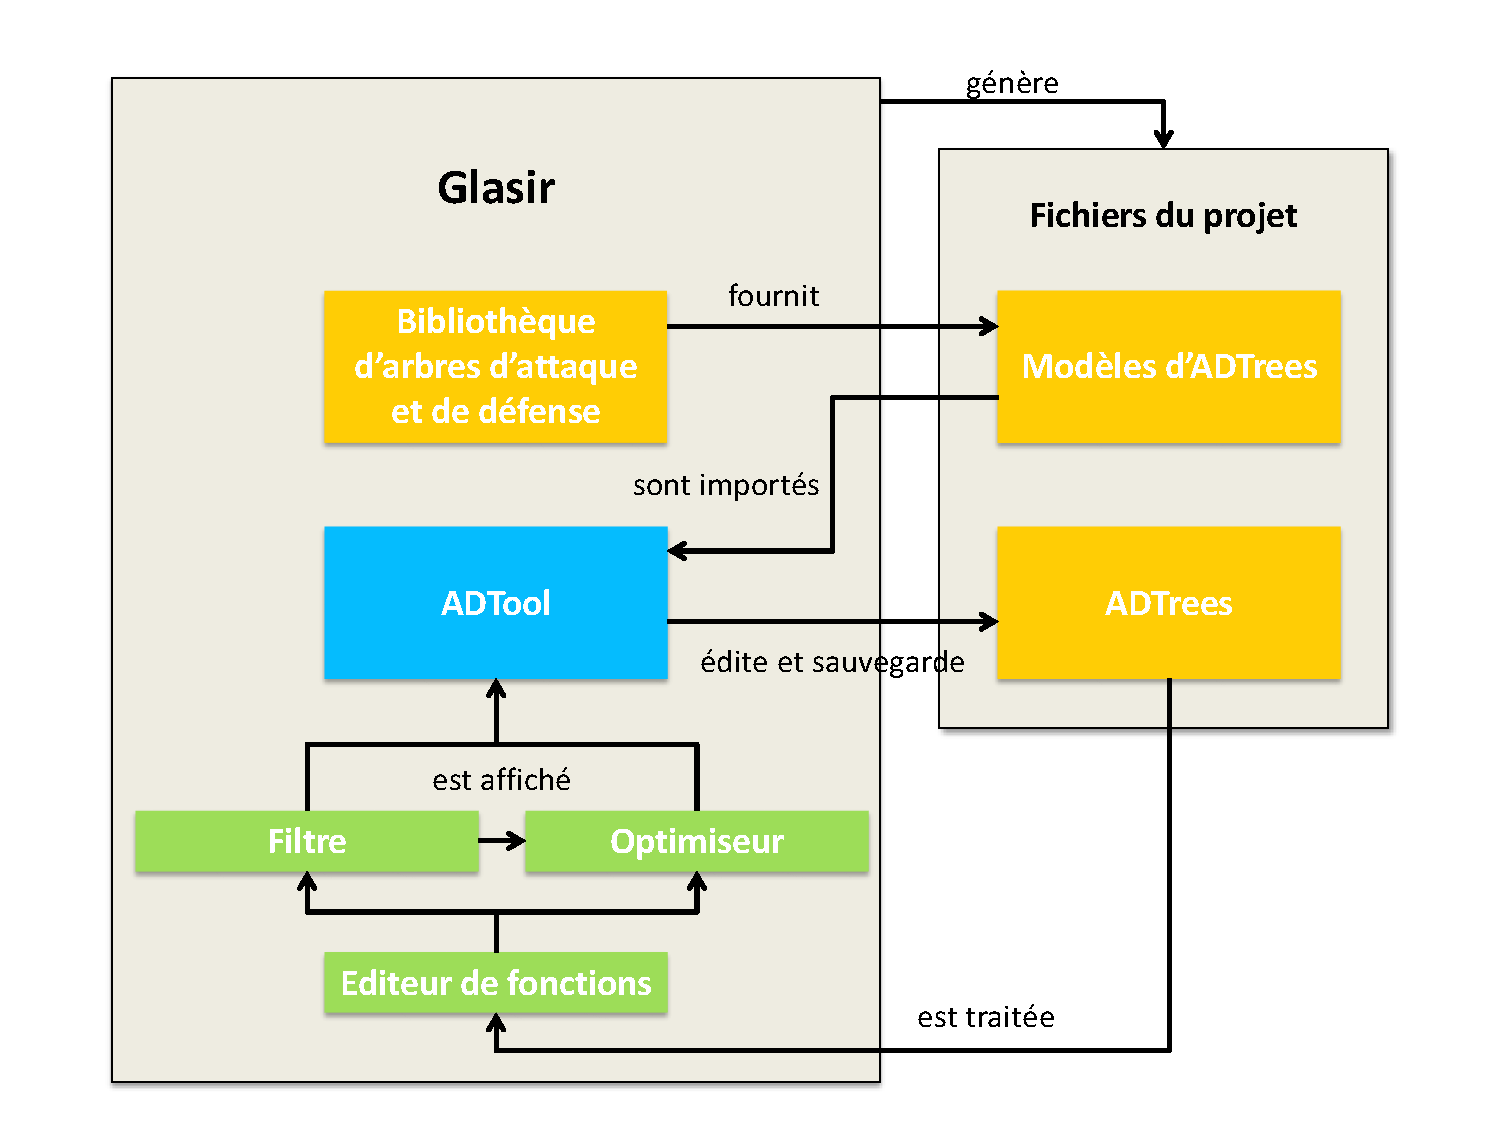
\includegraphics[width=0.8\textwidth]{figure/archiGlasir.pdf}
            \caption{Architecture initialement prévue.}
            \label{fig:archiPrevue}
        \end{figure}


		
        
        \begin{figure}[H]
            \centering
                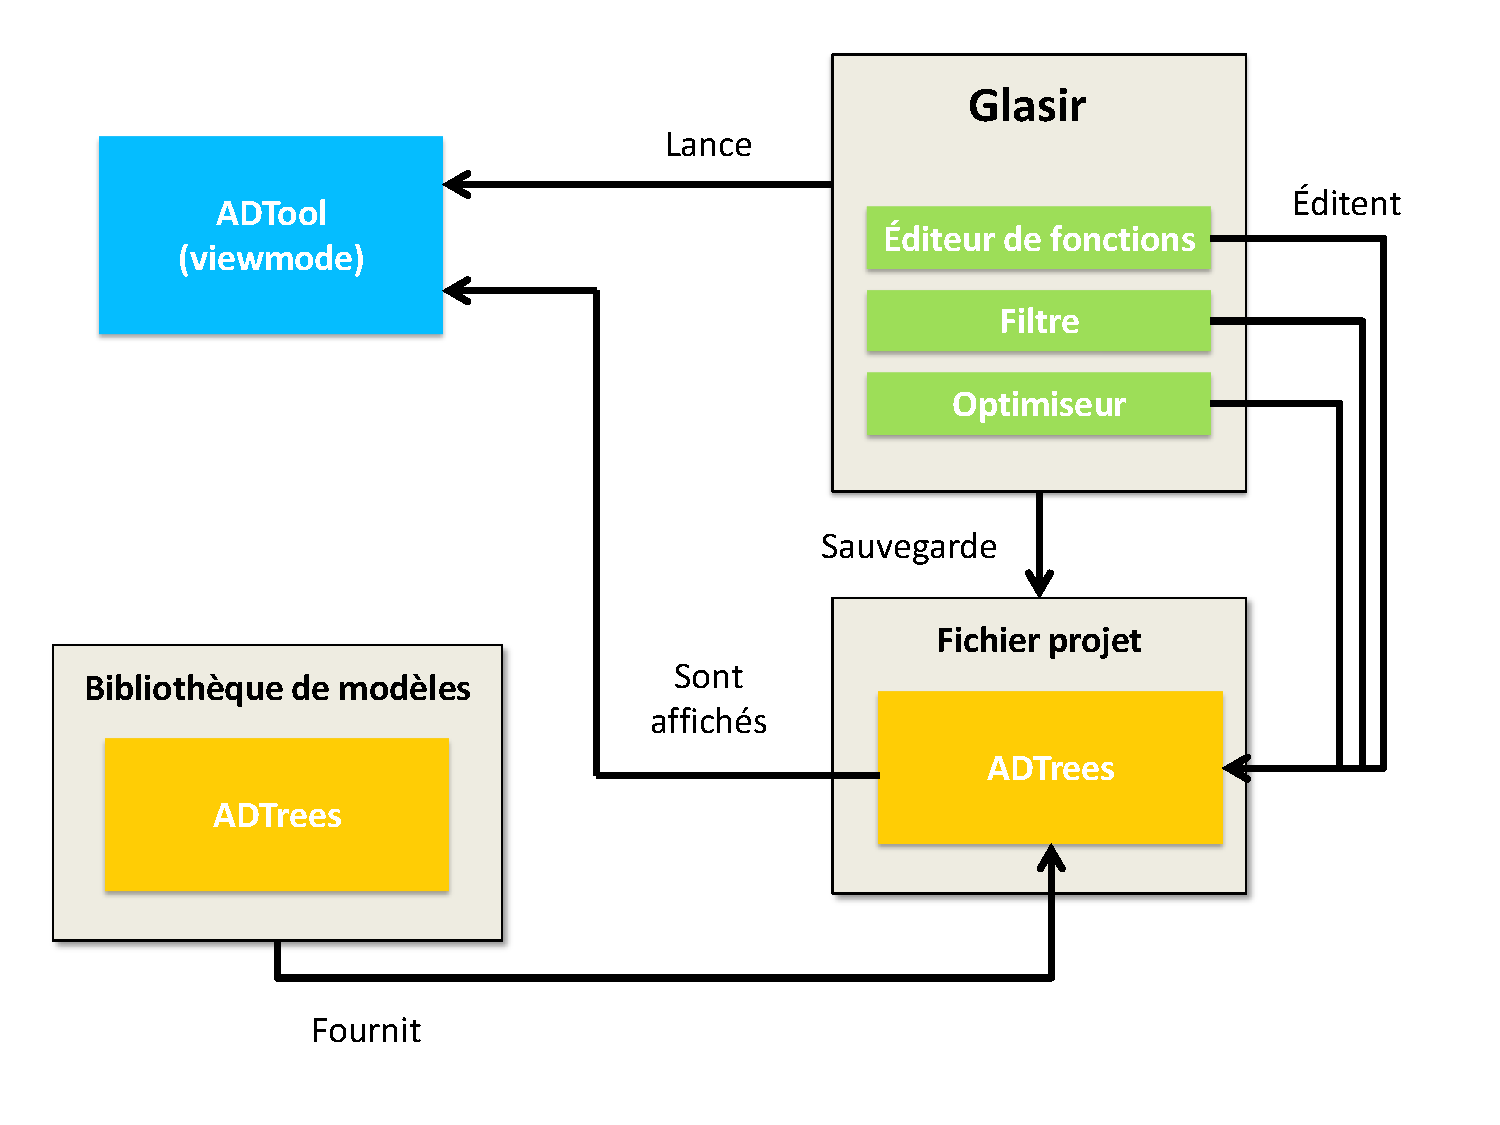
\includegraphics[width=0.8\textwidth]{figure/archiReelle.pdf}
            \caption{Architecture réelle.}
            \label{fig:archiReelle}
        \end{figure}
        

\newpage
\subsection{Rapport de conception}

La {\sc Figure} \ref{fig:copypastePrevu} illustre l'implémentation du copy-paste imaginée lors du rapport de conception. Pour des raisons techniques, l'implémentation du copy-paste est telle qu'indiqué sur la {\sc Figure} \ref{fig:copypasteReel}. De même, la {\sc Figure} \ref{fig:ctrlzPrevu} illustre l'implémentation du ctrl-z imaginée lors du rapport de conception, tandis la {\sc Figure} \ref{fig:ctrlzReel} indique son implémentation réelle.

		\begin{figure}[H]
            \centering
                
\includegraphics[width=0.8\textwidth]{figure/copiercoller.png}
            \caption{Diagramme de classe prévu pour le copier-coller.}
            \label{fig:copypastePrevu}
        \end{figure}
        
        \begin{figure}[H]
            \centering
                
\includegraphics[width=0.1\textwidth]{figure/liste.png}
            \caption{Diagramme de classe réel pour le copier-coller.}
            \label{fig:copypasteReel}
        \end{figure}
       
        \begin{figure}[H]
            \centering
                
\includegraphics[width=0.8\textwidth]{figure/ctrlz.png}
            \caption{Diagramme de classe prévu pour le ctrl-z.}
            \label{fig:ctrlzPrevu}
        \end{figure}
        
        \begin{figure}[H]
            \centering
                
\includegraphics[width=0.1\textwidth]{figure/liste.png}
            \caption{Diagramme de classe réel pour le ctrl-z.}
            \label{fig:ctrlzReel}
        \end{figure}

\newpage
\newpage